% Provenance (never printed): cycle 3 "La planete Terre. Les etres vivants
% dans leur environnement" (natural phenomena: volcanoes and earthquakes,
% natural hazards and the behaviour to adopt); see sources/book1/PROVENANCE.md.
% Book 1, grade 4, chapter 2.
\chapter{Vulcões e terremotos: um primeiro olhar}\label{ch:g4:volcanoes-earthquakes-first-look}

Na segunda-feira à noite, o telejornal mostra um \omterm{def:g4:volcanoes-earthquakes-first-look:volcano}{vulcão} numa ilha
distante. No escuro, um chafariz de \omterm{def:g3:stones-pebbles-sand:rock}{rocha} alaranjada e incandescente jorra
de uma rachadura no chão, e \omterm{def:g1:landscapes-around-us:water}{rios} de fogo descem devagar pela encosta até
o \omterm{def:g2:water-on-earth:ocean}{mar}, chiando e soltando vapor. Na quinta-feira, o telejornal mostra
outro lugar: uma cidadezinha onde, ao amanhecer, o chão tremeu durante
meio minuto. Chaminés caíram na rua, e uma casa velha escorregou da sua base.

São dois acontecimentos muito diferentes. Mas os dois vêm das profundezas
da Terra e, como vamos ver, os dois acontecem muito mais em certas partes
do mundo do que em outras.

\begin{recall}
\omterm{def:g1:landscapes-around-us:landform}{Montanhas}, \omterm{def:g1:landscapes-around-us:landform}{colinas}, \omterm{def:g1:landscapes-around-us:landform}{vales} e \omterm{def:g1:landscapes-around-us:landform}{planícies} são as formas do terreno
(\cref{ch:g1:landscapes-around-us}). As terras da Terra estão reunidas em
sete \omterm{def:g3:continents-and-oceans:continent}{continentes}, entre cinco \omterm{def:g2:water-on-earth:ocean}{oceanos}; o Pacífico é o maior \omterm{def:g2:water-on-earth:ocean}{oceano}
(\cref{ch:g3:continents-and-oceans}).
\end{recall}

\section{Um vulcão entra em erupção}

Lá no fundo, sob os nossos pés, a Terra é muito quente. Em alguns lugares,
a \omterm{def:g3:stones-pebbles-sand:rock}{rocha} lá embaixo está tão quente que derreteu. Essa \omterm{def:g3:stones-pebbles-sand:rock}{rocha} derretida é
mais leve que a \omterm{def:g3:stones-pebbles-sand:rock}{rocha} sólida em volta; por isso ela sobe devagar, como uma
rolha na água. Onde ela encontra uma saída para a superfície, nasce um \omterm{def:g4:volcanoes-earthquakes-first-look:volcano}{vulcão}.

\begin{definition}[Vulcão]\label{def:g4:volcanoes-earthquakes-first-look:volcano}
Um \emph{vulcão}\index{vulcao@vulcão} é um lugar onde a \omterm{def:g3:stones-pebbles-sand:rock}{rocha} derretida das
profundezas da Terra sai na superfície, e também a \omterm{def:g1:landscapes-around-us:landform}{colina} ou a \omterm{def:g1:landscapes-around-us:landform}{montanha}
que essa \omterm{def:g3:stones-pebbles-sand:rock}{rocha} derretida constrói ali, camada após camada.
\end{definition}

\begin{definition}[Erupção, lava e cinza vulcânica]\label{def:g4:volcanoes-earthquakes-first-look:eruption}
Uma \emph{erupção}\index{erupcao@erupção} é o momento em que um \omterm{def:g4:volcanoes-earthquakes-first-look:volcano}{vulcão} lança
\omterm{def:g3:stones-pebbles-sand:rock}{rocha} derretida, cinzas e gases. A \emph{lava}\index{lava} é a \omterm{def:g3:stones-pebbles-sand:rock}{rocha}
derretida que escorre pela superfície; ela corre, depois esfria e endurece,
formando \omterm{def:g3:stones-pebbles-sand:rock}{rocha} nova. A \emph{cinza vulcânica}\index{cinza vulcanica@cinza vulcânica} é feita de
pedacinhos minúsculos de \omterm{def:g3:stones-pebbles-sand:rock}{rocha} e de vidro lançados no ar por uma erupção;
ela cai de volta como uma \omterm{def:g4:clouds-rain-snow:precipitation}{neve} cinzenta.
\end{definition}

\begin{omfigure}
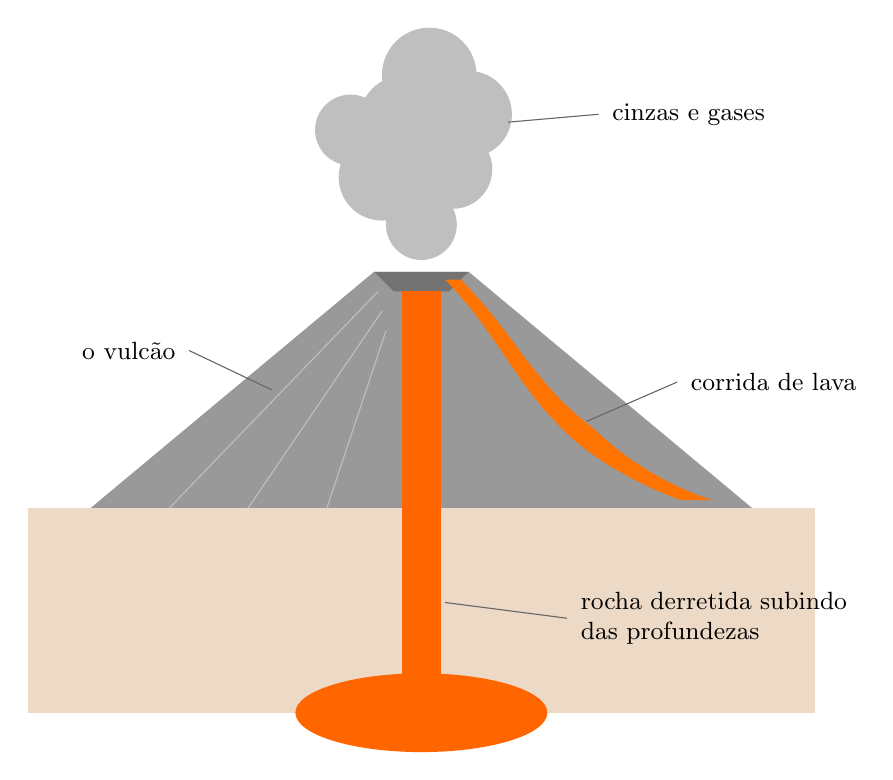
\begin{tikzpicture}[font=\small]
  % ground and deep rock
  \fill[brown!30] (-5,-2.6) rectangle (5,0);
  % the volcano
  \fill[black!40] (-4.2,0) -- (-0.6,3.0) -- (0.6,3.0) -- (4.2,0) -- cycle;
  \fill[black!55] (-0.6,3.0) -- (-0.35,2.75) -- (0.35,2.75) -- (0.6,3.0) -- cycle;
  % layers inside the cone
  \foreach \k in {1,2,3}
    \draw[black!25] (-4.2+1.0*\k,0) -- (-0.6+0.05*\k,3.0-0.25*\k);
  % molten rock rising from deep below
  \fill[orange!80!red] (-0.25,-2.6) -- (-0.25,2.75) -- (0.25,2.75) -- (0.25,-2.6) -- cycle;
  \fill[orange!80!red] (0,-2.6) ellipse (1.6 and 0.5);
  % lava flow on the right flank
  \fill[orange!90!red] (0.5,2.9) .. controls (1.2,2.2) and (1.4,1.6) .. (2.2,1.0)
    .. controls (2.6,0.6) and (3.2,0.25) .. (3.7,0.1) -- (3.3,0.1)
    .. controls (2.6,0.35) and (2.0,0.75) .. (1.7,1.1)
    .. controls (1.2,1.6) and (0.9,2.3) .. (0.3,2.9) -- cycle;
  % ash and gas cloud
  \foreach \x/\y/\r in {0/3.6/0.45, -0.5/4.2/0.55, 0.4/4.3/0.5, -0.2/4.9/0.6, 0.6/5.0/0.55, -0.9/4.8/0.45, 0.1/5.5/0.6}
    \fill[black!25] (\x,\y) circle (\r);
  % labels
  \node[anchor=west] at (2.3,5.0) {cinzas e gases};
  \draw[black!60] (2.25,5.0) -- (1.1,4.9);
  \node[anchor=west] at (3.3,1.6) {corrida de lava};
  \draw[black!60] (3.25,1.6) -- (2.1,1.1);
  \node[anchor=east] at (-3.0,2.0) {o vulcão};
  \draw[black!60] (-2.95,2.0) -- (-1.9,1.5);
  \node[anchor=west, align=left] at (1.9,-1.4) {rocha derretida subindo\\das profundezas};
  \draw[black!60] (1.85,-1.4) -- (0.3,-1.2);
\end{tikzpicture}

{\small Um \omterm{def:g4:volcanoes-earthquakes-first-look:volcano}{vulcão} em \omterm{def:g4:volcanoes-earthquakes-first-look:eruption}{erupção} (desenho, fora de escala). A \omterm{def:g3:stones-pebbles-sand:rock}{rocha} derretida
sobe das profundezas e sai no alto: ela desce como \omterm{def:g4:volcanoes-earthquakes-first-look:eruption}{lava}, enquanto as
cinzas e os gases são lançados para o céu. Cada \omterm{def:g4:volcanoes-earthquakes-first-look:eruption}{erupção} acrescenta uma
nova camada à \omterm{def:g1:landscapes-around-us:landform}{montanha}.}
\label{fig:g4:volcanoes-earthquakes-first-look:volcano}
\end{omfigure}

Nem todas as \omterm{def:g4:volcanoes-earthquakes-first-look:eruption}{erupções} são parecidas. Em algumas, a \omterm{def:g4:volcanoes-earthquakes-first-look:eruption}{lava} é fluida: ela
escorre tranquilamente em \omterm{def:g1:landscapes-around-us:water}{rios} incandescentes que podem correr por
quilômetros, às vezes até o \omterm{def:g2:water-on-earth:ocean}{mar}. Em outras, a \omterm{def:g3:stones-pebbles-sand:rock}{rocha} derretida é grossa e
cheia de gás, como uma garrafa de refrigerante sacudida: quando ela sai,
explode numa enorme coluna de cinzas que sobe bem alto no céu.

\begin{omfigure}
\begin{minipage}[b]{0.56\linewidth}\centering
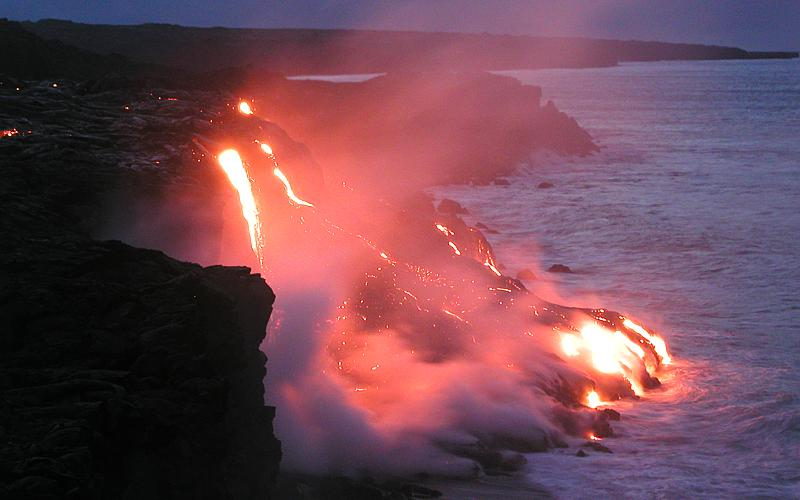
\includegraphics[width=\linewidth]{images/book1/g4-lava-ocean.jpg}

{\small Uma \omterm{def:g4:volcanoes-earthquakes-first-look:eruption}{erupção} de \omterm{def:g4:volcanoes-earthquakes-first-look:eruption}{lava} fluida: a \omterm{def:g4:volcanoes-earthquakes-first-look:eruption}{lava} desce por um penhasco à \omterm{def:g2:water-on-earth:ocean}{beira-mar}
até o \omterm{def:g2:water-on-earth:ocean}{oceano}, no Havaí. Foto: USGS Hawaiian Volcano Observatory (domínio público).}
\end{minipage}\hfill
\begin{minipage}[b]{0.4\linewidth}\centering
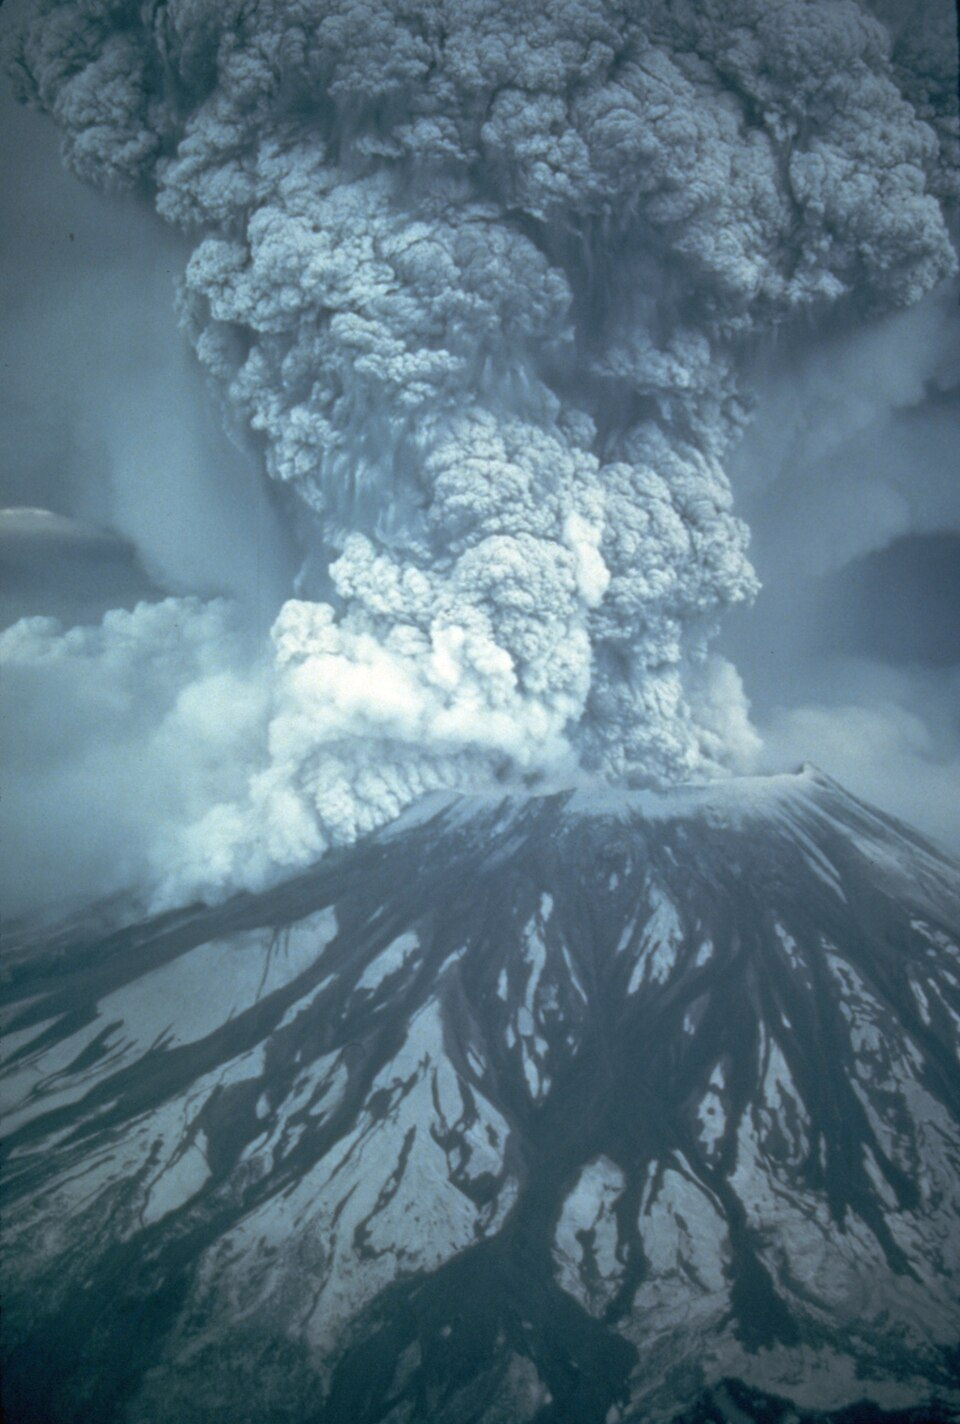
\includegraphics[width=0.78\linewidth]{images/book1/g4-st-helens.jpg}

{\small Uma \omterm{def:g4:volcanoes-earthquakes-first-look:eruption}{erupção} explosiva: o monte Santa Helena, Estados Unidos, 18~de
maio de 1980. Foto: Austin Post, USGS (domínio público).}
\end{minipage}
% ledger: usgs:pu-oo-ocean, usgs:msh-1980
\label{fig:g4:volcanoes-earthquakes-first-look:two-eruptions}
\end{omfigure}

\begin{example}[O monte Santa Helena, 1980]\label{ex:g4:volcanoes-earthquakes-first-look:st-helens}
Na primavera de 1980, um calombo cresceu na encosta do monte Santa Helena,
porque a \omterm{def:g3:stones-pebbles-sand:rock}{rocha} derretida empurrava para cima dentro da \omterm{def:g1:landscapes-around-us:landform}{montanha}. Na manhã
de 18~de maio, um pequeno \omterm{def:g4:volcanoes-earthquakes-first-look:earthquake}{terremoto} sacudiu a \omterm{def:g1:landscapes-around-us:landform}{montanha}, o calombo
escorregou num deslizamento gigante, e o \omterm{def:g4:volcanoes-earthquakes-first-look:volcano}{vulcão} explodiu para o lado e
para cima. Os 400~metros do topo da \omterm{def:g1:landscapes-around-us:landform}{montanha} sumiram: o cume virou uma
cratera enorme.
% ledger: usgs:msh-1980
\end{example}

\section{O chão treme}

As \omterm{def:g3:stones-pebbles-sand:rock}{rochas} lá no fundo, sob os nossos pés, não estão perfeitamente paradas.
Muito devagar, elas são empurradas e puxadas. Elas se curvam um pouco,
como uma régua que você empurra pelas duas pontas --- até que, de repente,
se quebram e escorregam. O tranco faz o chão tremer por quilômetros em volta.

\begin{definition}[Terremoto]\label{def:g4:volcanoes-earthquakes-first-look:earthquake}
Um \emph{terremoto}\index{terremoto} é um tremor repentino do chão, causado
por \omterm{def:g3:stones-pebbles-sand:rock}{rochas} que se quebram e escorregam, lá no fundo da terra.
\end{definition}

Um \omterm{def:g4:volcanoes-earthquakes-first-look:earthquake}{terremoto} costuma durar só alguns segundos, às vezes um ou dois minutos
para os maiores. A maioria dos \omterm{def:g4:volcanoes-earthquakes-first-look:earthquake}{terremotos} é tão pequena que ninguém sente:
só os instrumentos percebem. Um \omterm{def:g4:volcanoes-earthquakes-first-look:earthquake}{terremoto} forte pode fazer o chão balançar
como o convés de um navio, rachar estradas e derrubar muros e casas.

\begin{omfigure}
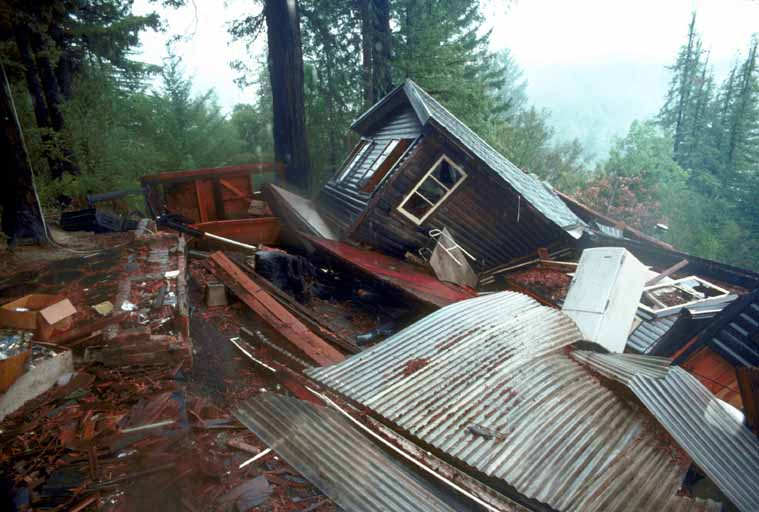
\includegraphics[width=0.55\linewidth]{images/book1/g4-loma-prieta-house.jpg}

{\small Depois de um \omterm{def:g4:volcanoes-earthquakes-first-look:earthquake}{terremoto} forte na Califórnia, em 1989: esta casa de
madeira foi jogada para o lado, para fora da sua base de concreto. Foto:
J.~K.~Nakata, USGS (domínio público).}
% ledger: usgs:loma-prieta-house
\end{omfigure}

\begin{remark}[Com que frequência?]\label{rem:g4:volcanoes-earthquakes-first-look:how-often}
Os geólogos mantêm uma lista de todos os grandes \omterm{def:g4:volcanoes-earthquakes-first-look:earthquake}{terremotos} da Terra. Nos
50 anos de 1976 a 2025, a lista conta 7\,031 \omterm{def:g4:volcanoes-earthquakes-first-look:earthquake}{terremotos} grandes (fortes o
bastante para danificar os prédios perto deles): cerca de 141 por ano, ou
quase 3 por semana. Os maiores de todos, que podem destruir cidades
inteiras, são cerca de 14 por ano. Nessa mesma Terra, cerca de 1\,200
\omterm{def:g4:volcanoes-earthquakes-first-look:volcano}{vulcões} entraram em \omterm{def:g4:volcanoes-earthquakes-first-look:eruption}{erupção} nos últimos doze mil anos, mais ou menos.
% ledger: data:usgs-comcat, data:gvp
\end{remark}

\section{Onde acontecem os vulcões e os terremotos}

Se os \omterm{def:g4:volcanoes-earthquakes-first-look:volcano}{vulcões} e os \omterm{def:g4:volcanoes-earthquakes-first-look:earthquake}{terremotos} acontecessem em qualquer lugar, ao acaso, os
pontos num \omterm{def:g3:continents-and-oceans:world-map}{mapa-múndi} estariam espalhados por igual. Não estão.

O \omterm{def:g2:drawing-to-map:map}{mapa} abaixo mostra um desenho impressionante. A maioria dos \omterm{def:g4:volcanoes-earthquakes-first-look:volcano}{vulcões} e dos
grandes \omterm{def:g4:volcanoes-earthquakes-first-look:earthquake}{terremotos} fica em faixas compridas e estreitas. A mais comprida
de todas dá a volta no \omterm{def:g2:water-on-earth:ocean}{oceano} Pacífico: da Nova Zelândia, sobe pela
Indonésia, pelas Filipinas e pelo Japão, passa pelo Alasca e depois desce
por toda a costa oeste das Américas até a ponta do Chile. Por causa dos
seus muitos \omterm{def:g4:volcanoes-earthquakes-first-look:volcano}{vulcões}, ela é muitas vezes chamada de ``Círculo de Fogo''.

\begin{example}[Contando no mapa]\label{ex:g4:volcanoes-earthquakes-first-look:shares}
Contamos os pontos que ficam no anel sombreado (a menos de
500~quilômetros da sua linha central). Dos 1\,214 \omterm{def:g4:volcanoes-earthquakes-first-look:volcano}{vulcões}, 837 estão no
anel: cerca de 2 em cada 3. Dos 696 \omterm{def:g4:volcanoes-earthquakes-first-look:earthquake}{terremotos} muito grandes, 532 estão no
anel: cerca de 3 em cada 4. O anel cobre só uma pequena parte da Terra,
mas guarda a maioria dos seus \omterm{def:g4:volcanoes-earthquakes-first-look:volcano}{vulcões} e \omterm{def:g4:volcanoes-earthquakes-first-look:earthquake}{terremotos}.
% ledger: data:gvp, data:usgs-comcat
\end{example}

\begin{omfigure}
\begin{tikzpicture}
\begin{axis}[ommap, width=\linewidth, xtick=\empty, ytick=\empty, grid=none,
    legend style={font=\scriptsize, at={(0.5,-0.02)}, anchor=north,
      draw=none, legend columns=3, /tikz/every even column/.append style={column sep=6pt}},
    legend cell align=left]
  \addplot[fill=omHypsLandA!85!black, draw=black!45, line width=0.2pt, forget plot]
    table {figdata/out/shared-geo-land.dat};
  \addplot[orange!80!black, opacity=0.35, line width=9pt, line cap=round, line join=round]
    table {figdata/out/grade-4-ring_of_fire-ring.dat};
  \addlegendentry{o anel em volta do Pacífico}
  \addplot[only marks, mark=triangle*, mark size=1.3pt, red!75!black]
    table[x=lon, y=lat] {figdata/out/grade-4-ring_of_fire-volcanoes.dat};
  \addlegendentry{um vulcão (últimos 12\,000 anos)}
  \addplot[only marks, mark=*, mark size=1.0pt, black, fill opacity=0.6]
    table[x=lon, y=lat] {figdata/out/grade-4-ring_of_fire-quakes7.dat};
  \addlegendentry{um terremoto muito grande (1976--2025)}
\end{axis}
\end{tikzpicture}

{\small Os \omterm{def:g4:volcanoes-earthquakes-first-look:volcano}{vulcões} que entraram em \omterm{def:g4:volcanoes-earthquakes-first-look:eruption}{erupção} nos últimos doze mil anos, mais ou
menos, e os maiores \omterm{def:g4:volcanoes-earthquakes-first-look:earthquake}{terremotos} de 1976--2025. A maioria deles fica ao longo
de um anel de cadeias de ilhas e de cordilheiras em volta do \omterm{def:g2:water-on-earth:ocean}{oceano}
Pacífico (sombreado). Dados: Smithsonian Global Volcanism Program;
catálogo de \omterm{def:g4:volcanoes-earthquakes-first-look:earthquake}{terremotos} do Serviço Geológico dos Estados Unidos (USGS);
contornos das costas: Natural Earth.}
\label{fig:g4:volcanoes-earthquakes-first-look:map}
% ledger: data:gvp, data:usgs-comcat, data:ne-land
\end{omfigure}

Outras faixas são menores: uma atravessa o sul da Europa e da Ásia, do \omterm{def:g2:water-on-earth:ocean}{mar}
Mediterrâneo até o Himalaia; outras passam pelo meio dos \omterm{def:g2:water-on-earth:ocean}{oceanos}, onde os
\omterm{def:g4:volcanoes-earthquakes-first-look:volcano}{vulcões} ficam escondidos embaixo da água. Alguns lugares, como o Havaí,
têm \omterm{def:g4:volcanoes-earthquakes-first-look:volcano}{vulcões} longe de qualquer faixa. Por que as faixas estão onde estão é
uma pergunta para o \cref{ch:g7:plate-tectonics}: a resposta explica a forma do \omterm{def:g2:drawing-to-map:map}{mapa} inteiro.

\section{Como se proteger}

Ninguém consegue impedir uma \omterm{def:g4:volcanoes-earthquakes-first-look:eruption}{erupção} ou um \omterm{def:g4:volcanoes-earthquakes-first-look:earthquake}{terremoto}. Mas saber o que
fazer salva vidas.

\begin{omfigure}
\begin{tikzpicture}[font=\small, line cap=round, line join=round]
  % --- panel 1: DROP onto hands and knees
  \begin{scope}
    \draw[black!30] (-0.2,0) -- (2.8,0);
    \fill[omDef] (0.62,0.98) circle (0.21);
    \draw[omDef, line width=2.2pt] (0.88,0.98) -- (2.0,0.95);
    \draw[omDef, line width=2pt] (0.95,0.96) -- (0.95,0.05);
    \draw[omDef, line width=2pt] (2.0,0.95) -- (1.98,0.08) -- (2.65,0.08);
    \node[font=\bfseries] at (1.3,-0.45) {ABAIXE-SE};
    \node[font=\scriptsize, align=center] at (1.3,-0.95) {fique de quatro,\\com as mãos no chão};
  \end{scope}
  % --- panel 2: COVER under a table
  \begin{scope}[xshift=4cm]
    \draw[black!30] (-0.2,0) -- (2.8,0);
    \fill[brown!60!black] (-0.1,1.45) rectangle (2.7,1.6);
    \draw[brown!60!black, line width=2pt] (0.1,1.45) -- (0.1,0) (2.5,1.45) -- (2.5,0);
    \fill[omDef] (0.75,0.95) circle (0.2);
    \draw[omDef, line width=2.2pt] (0.95,0.85) -- (1.95,0.8);
    \draw[omDef, line width=2pt] (1.9,0.8) -- (1.65,0.05) -- (2.25,0.05);
    \draw[omDef, line width=2pt] (1.0,0.85) -- (0.7,1.2) -- (0.5,0.95);
    \node[font=\bfseries] at (1.3,-0.45) {PROTEJA-SE};
    \node[font=\scriptsize, align=center] at (1.3,-0.95) {cubra a cabeça e o pescoço,\\sob uma mesa resistente};
  \end{scope}
  % --- panel 3: HOLD ON to the table leg
  \begin{scope}[xshift=8cm]
    \draw[black!30] (-0.2,0) -- (2.8,0);
    \fill[brown!60!black] (-0.1,1.45) rectangle (2.7,1.6);
    \draw[brown!60!black, line width=2pt] (0.1,1.45) -- (0.1,0) (2.5,1.45) -- (2.5,0);
    \fill[omDef] (0.75,0.95) circle (0.2);
    \draw[omDef, line width=2.2pt] (0.95,0.85) -- (1.95,0.8);
    \draw[omDef, line width=2pt] (1.9,0.8) -- (1.65,0.05) -- (2.25,0.05);
    \draw[omDef, line width=2pt] (1.0,0.85) -- (0.7,1.2) -- (0.5,0.95);
    \draw[omDef, line width=2pt] (1.0,0.8) -- (0.45,0.6) -- (0.12,0.65);
    \node[font=\bfseries] at (1.3,-0.45) {SEGURE-SE};
    \node[font=\scriptsize, align=center] at (1.3,-0.95) {na mesa até o\\tremor parar};
  \end{scope}
\end{tikzpicture}

{\small O que fazer assim que o chão começa a tremer: abaixar-se,
proteger-se e segurar-se.}
\label{fig:g4:volcanoes-earthquakes-first-look:drop-cover}
% ledger: shakeout:dch
\end{omfigure}

\begin{safety}
\textbf{Num \omterm{def:g4:volcanoes-earthquakes-first-look:earthquake}{terremoto}.} Assim que sentir o chão tremer: \textbf{abaixe-se}
e fique de quatro; \textbf{proteja} a cabeça e o pescoço com o braço e
engatinhe para baixo de uma mesa ou carteira resistente, se houver uma
perto; \textbf{segure-se} nela até o tremor parar. Não saia correndo para
fora enquanto o chão treme, e não fique parado no vão de uma porta: os
vidros e os objetos que caem são o principal perigo. Quando o tremor
parar, saia do prédio com calma, como você treina nos simulados da escola.

\textbf{Perto de um \omterm{def:g4:volcanoes-earthquakes-first-look:volcano}{vulcão}.} Os cientistas vigiam os \omterm{def:g4:volcanoes-earthquakes-first-look:volcano}{vulcões} que podem
despertar. Se eles avisam que uma \omterm{def:g4:volcanoes-earthquakes-first-look:eruption}{erupção} está para acontecer, as
autoridades mandam as pessoas sair da região. Siga as instruções na mesma
hora, e nunca chegue mais perto para olhar.
\end{safety}
% ledger: shakeout:dch

\begin{omfigure}

\includegraphics[width=0.55\linewidth]{images/book1/ai/g4-earthquake-drill.jpg}

{\small Um simulado de \omterm{def:g4:volcanoes-earthquakes-first-look:earthquake}{terremoto}: os alunos treinam ``abaixar-se,
proteger-se e segurar-se'' embaixo das carteiras.}
\end{omfigure}

\section{Exercícios}

\begin{exercise}[$\star$]\label{exo:g4:volcanoes-earthquakes-first-look:1}
\omterm{def:g4:volcanoes-earthquakes-first-look:eruption}{Lava}, cinza ou gás? (a) um \omterm{def:g1:landscapes-around-us:water}{rio} de \omterm{def:g3:stones-pebbles-sand:rock}{rocha} derretida incandescente descendo
uma encosta; (b) pedacinhos minúsculos de \omterm{def:g3:stones-pebbles-sand:rock}{rocha} lançados no céu, que caem de
volta como \omterm{def:g4:clouds-rain-snow:precipitation}{neve} cinzenta; (c) uma coisa invisível que escapa do \omterm{def:g4:volcanoes-earthquakes-first-look:volcano}{vulcão}
junto com as cinzas.
\end{exercise}

\begin{exercise}[$\star$]\label{exo:g4:volcanoes-earthquakes-first-look:2}
O que é um \omterm{def:g4:volcanoes-earthquakes-first-look:earthquake}{terremoto}? Ele dura horas ou segundos?
\end{exercise}

\begin{exercise}[$\star$]\label{exo:g4:volcanoes-earthquakes-first-look:3}
Coloque os três passos em ordem: segure-se; abaixe-se; proteja-se.
\end{exercise}

\begin{exercise}[$\star$]\label{exo:g4:volcanoes-earthquakes-first-look:4}
No \omterm{def:g2:drawing-to-map:map}{mapa} da página~\pageref{fig:g4:volcanoes-earthquakes-first-look:map}, em volta de
que \omterm{def:g2:water-on-earth:ocean}{oceano} fica a maioria dos \omterm{def:g4:volcanoes-earthquakes-first-look:volcano}{vulcões}?
\end{exercise}

\begin{exercise}[$\star$]\label{exo:g4:volcanoes-earthquakes-first-look:5}
Verdadeiro ou falso? (a) A maioria dos \omterm{def:g4:volcanoes-earthquakes-first-look:earthquake}{terremotos} é pequena demais para ser
sentida. (b) A \omterm{def:g4:volcanoes-earthquakes-first-look:eruption}{lava} continua líquida para sempre. (c) Quando o chão treme,
o mais seguro é sair correndo para fora.
\end{exercise}

\begin{exercise}[$\star$]\label{exo:g4:volcanoes-earthquakes-first-look:6}
Observe o desenho do \omterm{def:g4:volcanoes-earthquakes-first-look:volcano}{vulcão} na página~\pageref{fig:g4:volcanoes-earthquakes-first-look:volcano}.
De onde vem a \omterm{def:g3:stones-pebbles-sand:rock}{rocha} derretida? Por onde ela sai?
\end{exercise}

\begin{exercise}[$\star\star$]\label{exo:g4:volcanoes-earthquakes-first-look:7}
No \omterm{def:g2:drawing-to-map:map}{mapa}, encontre: (a) um país das Américas com muitos \omterm{def:g4:volcanoes-earthquakes-first-look:volcano}{vulcões} ao longo de
todo o seu comprimento; (b) um grupo de ilhas no meio do \omterm{def:g2:water-on-earth:ocean}{oceano} Pacífico,
com \omterm{def:g4:volcanoes-earthquakes-first-look:volcano}{vulcões}, que não fica no anel.
\end{exercise}

\begin{exercise}[$\star\star$]\label{exo:g4:volcanoes-earthquakes-first-look:8}
Acontecem cerca de 141 \omterm{def:g4:volcanoes-earthquakes-first-look:earthquake}{terremotos} grandes por ano. Mais ou menos quantos
isso dá por mês? (Um ano tem 12 meses; dê um número inteiro.)
\end{exercise}

\begin{exercise}[$\star\star$]\label{exo:g4:volcanoes-earthquakes-first-look:9}
Cerca de 3 em cada 4 \omterm{def:g4:volcanoes-earthquakes-first-look:earthquake}{terremotos} muito grandes acontecem no anel em volta do
Pacífico. De 20 \omterm{def:g4:volcanoes-earthquakes-first-look:earthquake}{terremotos} muito grandes, mais ou menos quantos você
esperaria no anel? E fora dele?
\end{exercise}

\begin{exercise}[$\star\star$]\label{exo:g4:volcanoes-earthquakes-first-look:10}
Durante um simulado de \omterm{def:g4:volcanoes-earthquakes-first-look:earthquake}{terremoto}, Leo corre para ficar no vão da porta da
sala. O que ele deveria ter feito, e por quê?
\end{exercise}

\begin{exercise}[$\star\star\star$]\label{exo:g4:volcanoes-earthquakes-first-look:11}
Dos 1\,214 \omterm{def:g4:volcanoes-earthquakes-first-look:volcano}{vulcões} do \omterm{def:g2:drawing-to-map:map}{mapa}, 837 estão no anel em volta do Pacífico. Quantos
estão fora dele? ``Cerca de 2 em 3'' é um bom jeito de descrever a parte
que está no anel? (Dica: quanto é dois terços de 1\,200?)
\end{exercise}
